\section{Ponto}

\texttt{point} é um \texttt{complex<T>}: \texttt{p.x} e \texttt{p.y} são as coordenadas, soma e subtração são de
vetores e \texttt{norm(p)} $= x^2 + y^2$. Com \texttt{T} inteiro os testes são exatos; com \texttt{T} real dá para
construir pontos novos (interseções, projeções).

\subsection*{Produto escalar e vetorial}

\smallskip{\centering
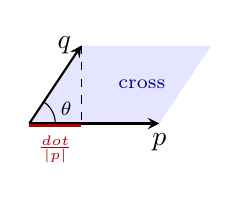
\begin{tikzpicture}[scale=0.55, >=stealth]
  \fill[blue!10] (0,0) -- (3,0) -- (4.2,1.8) -- (1.2,1.8) -- cycle;
  \draw[->, thick] (0,0) -- (3,0) node[below] {$p$};
  \draw[->, thick] (0,0) -- (1.2,1.8) node[left] {$q$};
  \draw[dashed] (1.2,1.8) -- (1.2,0);
  \draw[red!70!black, very thick] (0,-0.05) -- (1.2,-0.05);
  \node[red!70!black, below] at (0.6,-0.05) {\scriptsize $\frac{\text{dot}}{|p|}$};
  \draw (0.6,0) arc (0:56:0.6);
  \node at (0.85,0.35) {\scriptsize $\theta$};
  \node[blue!60!black] at (2.6,0.9) {\scriptsize cross};
\end{tikzpicture}
\par}\smallskip

\begin{itemize}
  \item \texttt{dot(p, q)} $= p_x q_x + p_y q_y = |p||q|\cos\theta$: a sombra de $q$ sobre $p$, vezes $|p|$.
        Positivo se o ângulo é agudo, zero se perpendicular, negativo se obtuso.
  \item \texttt{cross(p, q)} $= p_x q_y - p_y q_x = |p||q|\sin\theta$: a área com sinal do paralelogramo.
        Positivo se $q$ está à esquerda de $p$ (sentido anti-horário), zero se paralelos.
\end{itemize}

\subsection*{Orientação}

\smallskip{\centering
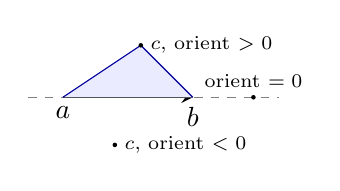
\begin{tikzpicture}[scale=0.55, >=stealth]
  \draw[gray, dashed] (-0.8,0) -- (5,0);
  \draw[->, thick] (0,0) -- (3,0);
  \node[below] at (0,0) {$a$};
  \node[below] at (3,0) {$b$};
  \fill[blue!8] (0,0) -- (1.8,1.2) -- (3,0) -- cycle;
  \draw[blue!60!black] (0,0) -- (1.8,1.2) -- (3,0);
  \fill (1.8,1.2) circle (1.5pt) node[right] {\scriptsize $c$, orient $> 0$};
  \fill (1.2,-1.1) circle (1.5pt) node[right] {\scriptsize $c$, orient $< 0$};
  \fill (4.4,0) circle (1.5pt) node[above] {\scriptsize orient $= 0$};
\end{tikzpicture}
\par}\smallskip

\texttt{orient(a, b, c)} $=$ \texttt{cross(b - a, c - a)}: positivo se $c$ está à esquerda da reta $a \to b$,
negativo se está à direita e zero se os três são colineares. A área do triângulo $abc$ é $|\text{orient}| / 2$.

\subsection*{perp, rotate e angle}

\smallskip{\centering
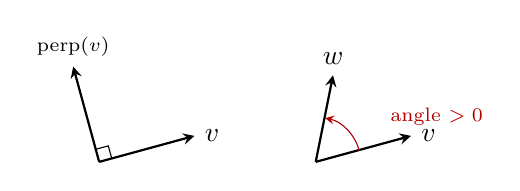
\begin{tikzpicture}[scale=0.55, >=stealth]
  \draw[->, thick] (0,0) -- (2.2,0.6) node[right] {$v$};
  \draw[->, thick] (0,0) -- (-0.6,2.2) node[above] {\scriptsize perp$(v)$};
  \draw (0.29,0.08) -- (0.21,0.37) -- (-0.08,0.29);
  \draw[->, thick] (5,0) -- (7.2,0.6) node[right] {$v$};
  \draw[->, thick] (5,0) -- (5.4,2.0) node[above] {$w$};
  \draw[->, red!70!black] (6,0.27) arc (15:78:1.03);
  \node[red!70!black, right] at (6.5,1.05) {\scriptsize angle $> 0$};
\end{tikzpicture}
\par}\smallskip

\texttt{perp(p)} $= (-y, x)$ gira $p$ em $90^\circ$ no sentido anti-horário, e \texttt{rotate(p, a)} gira $p$ em $a$ radianos (só com \texttt{T} real). \texttt{angle(v, w)} é o ângulo com
sinal de $v$ até $w$, em $[-\pi, \pi]$: negativo quando $w$ está à direita de $v$.

\subsection*{sign e dist2}

\texttt{sign(v)} devolve $-1$, $0$ ou $1$; com \texttt{T} real, valores em $[-10^{-9}, 10^{-9}]$ contam como zero.
Use sempre \texttt{sign} ao comparar com zero. O \texttt{==} entre pontos também usa \texttt{sign} em cada coordenada, então pontos construídos que deveriam coincidir são iguais. \texttt{dist2(a, b)} $= |a - b|^2$, exato com inteiros; a
distância é \texttt{sqrt(dist2(a, b))}.

\subsection*{Ordenação polar}

\smallskip{\centering
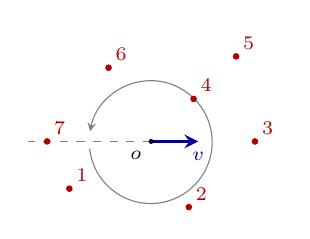
\begin{tikzpicture}[scale=0.6, >=stealth]
  \draw[gray, dashed] (0,0) -- (-2.6,0);
  \draw[->, very thick, blue!60!black] (0,0) -- (1,0) node[below] {\scriptsize $v$};
  \draw[->, gray] (-1.3,-0.15) arc (186:530:1.3);
  \fill (0,0) circle (1.5pt) node[below left] {\scriptsize $o$};
  \foreach \p/\k in {(-1.73,-1)/1, (0.8,-1.39)/2, (2.2,0)/3, (0.9,0.9)/4, (1.8,1.8)/5, (-0.9,1.56)/6, (-2.2,0)/7}
    \fill[red!70!black] \p circle (2pt) node[above right=-1pt] {\scriptsize \k};
\end{tikzpicture}
\par}\smallskip

\texttt{polar\_sort(p, o, v)} ordena os pontos pelo ângulo em torno de $o$, no sentido anti-horário, começando logo
depois da direção oposta a $v$ (tracejada). \texttt{is\_upper} separa as duas metades (o lado esquerdo de $v$, junto
com a direção oposta, vem depois) e, dentro de cada metade, o \texttt{cross} decide a ordem; pontos na mesma direção
saem do mais perto para o mais longe, como 4 e 5. Exato com \texttt{T} inteiro, sem \texttt{atan2}.

\subsection*{Par mais próximo}

\smallskip{\centering
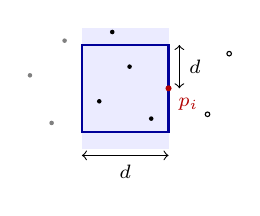
\begin{tikzpicture}[scale=0.55]
  \fill[blue!8] (1.5,-0.2) rectangle (3.5,2.6);
  \draw[blue!60!black, thick] (1.5,0.2) rectangle (3.5,2.2);
  \draw[<->] (1.5,-0.35) -- (3.5,-0.35) node[midway, below] {\scriptsize $d$};
  \draw[<->] (3.75,1.2) -- (3.75,2.2) node[midway, right] {\scriptsize $d$};
  \foreach \p in {(0.3,1.5), (0.8,0.4), (1.1,2.3)} \fill[gray] \p circle (1.5pt);
  \foreach \p in {(1.9,0.9), (2.6,1.7), (3.1,0.5)} \fill \p circle (1.5pt);
  \fill (2.2,2.5) circle (1.5pt);
  \fill[red!70!black] (3.5,1.2) circle (2pt) node[below right] {\scriptsize $p_i$};
  \foreach \p in {(4.4,0.6), (4.9,2.0)} \draw \p circle (1.5pt);
\end{tikzpicture}
\par}\smallskip

Percorre os pontos por $x$ guardando $d^2$, a menor distância ao quadrado até agora. Os ativos (faixa azul) são os
pontos com $x \ge x_i - d$, ordenados por $y$; os cinzas já saíram e os vazados ainda não entraram. Para $p_i$ só
testa os ativos no retângulo de altura $2d$, que são $O(1)$, então o total é $O(n \log n)$. Devolve
$\{d^2, i, j\}$, com os índices na entrada.
